\documentclass[12pt]{scrartcl}
\usepackage{graphicx}
\usepackage[default]{opensans}
\usepackage{sfmath} % sans font also for math
 \usepackage[binary-units = true]{siunitx}

% defining the paper layout that no text overlaps with the header
\usepackage[
  top=35mm,
  headheight=25mm,
  headsep=3mm,
  bottom=30mm,
  left=25mm,
  right=25mm
]{geometry}

\usepackage{latexsym}
\usepackage[centertags]{amsmath}
\usepackage{amssymb}

% custom header and footpage
\usepackage{scrpage2}
\pagestyle{scrheadings} % you have to set the custom layout
% Head
\ihead{M4.1: Simulation modules and interfaces } % left head
%\chead{}
\ohead{
\includegraphics[height=25mm]{EUCALL.png}}
% Foot
\ifoot{
\includegraphics[height=13.4mm]{EU.png}} % left foot
\cfoot{%
  \begin{minipage}{100mm}%
    \begin{scriptsize}%
      \normalfont{This project has received funding from the}
      \textit{European Union’s Horizon 2020 research and innovation programme}
      \normalfont{under grant agreement No 654220.}
    \end{scriptsize}%
  \end{minipage}%
} % center foot
\ofoot{\thepage} % right foot

\usepackage{booktabs}

% sophisticated linking of references in the pdf and setting some options
\usepackage{url}                                                  % for correct typesettings of URLs
\usepackage{hyperref}                                             % for sophisticated linking of urls, dois, pictures, tables, etc.
\hypersetup{
    unicode=true,                                                 % non-Latin characters in Acrobat’s bookmarks
    pdftoolbar=true,                                              % show Acrobat’s toolbar?
    pdfmenubar=true,                                              % show Acrobat’s menu?
    pdffitwindow=false,                                           % window fit to page when opened
    pdfstartview={FitH},                                          % fits the width of the page to the window
    pdftitle={M4.1: Simulation modules and interfaces},           % title
    pdfauthor={C. Fortmann-Grote},                                % author
    pdfsubject={EUCALL WP4 (SIMEX) Milestone 4.1},                % subject of the document
    pdfcreator={pdflatex},                                        % creator of the document
    pdfkeywords={EUCALL, SIMEX, simulations, PIC, XFEL, scattering},                                         % list of keywords
    pdfnewwindow=true,                                           % links in new PDF window
    colorlinks=true,                                             % false: boxed links; true: colored links
    linkcolor=blue,                                              % color of internal links (change box color with linkbordercolor)
    citecolor=blue,                                              % color of links to bibliography
    filecolor=blue,                                              % color of file links
    urlcolor=blue                                                % color of external links
}

% Zeilenabstand
\renewcommand{\baselinestretch}{1.2}


%%%%%%%%%%%%%%%%%%%%%%%%%%%%%%%%%%%%%%%%%%%%%%%
%   BIBLIOGRAPHY SETTINGS                     %
%%%%%%%%%%%%%%%%%%%%%%%%%%%%%%%%%%%%%%%%%%%%%%%
\usepackage[bibstyle=nature,sorting=none,=maxnames=1000,eprint=false,
defernumbers=true, backend=biber]{biblatex}
\usepackage{hyperref}

\renewcommand*\finalnamedelim{, and\addspace}
\DeclareNameAlias{sortname}{last-first}
\renewcommand{\newunitpunct}{, }

\AtEveryBibitem{%
  \clearfield{day}%
  \clearfield{month}%
  \clearfield{endday}%
  \clearfield{endmonth}%
  \clearfield{issn}%
  \clearfield{issue}%
}
%convert titles to hyperlinks using doi
\ExecuteBibliographyOptions{doi=false} \newbibmacro{string+doi}[1]{%
  \iffieldundef{doi}{#1}{\href{http://dx.doi.org/\thefield{doi}}{#1}}}
  \DeclareFieldFormat*{title}{\usebibmacro{string+doi}{\mkbibemph{#1}}}

%\addbibresource{/home/grotec/Documents/LiteratureDB/bibtex/jabref.bib}
\addbibresource{references.bib}
%%%%%%%%%%%%%%%%%%%%%%%%%%%%%%%%%%%%%%%%%%%%%%%
% END BIBLIOGRAPHY SETTINGS                   %
%%%%%%%%%%%%%%%%%%%%%%%%%%%%%%%%%%%%%%%%%%%%%%%

\begin{document}
\makeatletter
\begin{titlepage}
\thispagestyle{scrheadings}
\begin{center}
$~$\\
\vspace{2cm}
\Huge{\textbf{WP 4 -- SIMEX\\[1cm]
Milestone M4.1: Delivery of individual simulation modules and common interfaces
for interoperability}}\\[5mm]
\vspace{2cm}
\large{
Carsten Fortmann-Grote, Alexander Andreev, Richard Briggs,\\ Michael Bussmann,
  Axel Huebl, Thomas Kluge,\\
 S. Pascarelli, Ashutosh Sharma, and Adrian P. Mancuso\\
 }
\vspace{1cm}
\@date
\end{center}
\vfill%

\includegraphics[width=\textwidth]{PartnerLogos.pdf}
\normalfont
\end{titlepage}
\makeatother
%
\tableofcontents
%
\newpage
%
\section{Introduction}
The computer program \texttt{simex\_platform} \cite{simex_github} is a modular
software environment for the simulation of experiments at advanced laser light
sources. Users can assemble a virtual experiment through the combination
of suitable simulation codes for the various instrumental parts of the
experiment: the light source (e.g. a synchrotron, an x-ray free
electron laser), propagation of radiation from the source to the
point of interaction with a sample or target, interaction of the light with the sample,
propagation of the scattered and trasmitted light after the
interaction, and detection. We have equipped \texttt{simex\_platform}
with a number of such codes and user interfaces to ease setup and execution of
simulation runs. A lightweight abstraction mechanism and interface templates
makes the integration of further simulation codes straightforward, so users can
include their own or 3rd party simulation codes in the framework.
In this way, they can embed their codes
into a more realistic simulation environment compared to running codes isolated
with more or less idealized parameters and initial conditions.

\subsection{The EUCALL Software repository}
The central access point for all codes, scripts, and documentation in SIMEX is
the EUCALL software repository at
\url{https://github.com/eucall-software}. The repository hosts
the code for \texttt{simex\_platform} at
\url{https://github.com/eucall-software/simex\_platform} next to a number of code
projects for various simulation tasks, e.g. short-pulse laser matter interaction
(\url{https://github.com/eucall-software/picongpu}) and coherent diffraction
(\url{https://github.com/eucall-software/singfel}). The repository is
also used for non-software collaborative projects, e.g. publication manuscripts
and presentations.
%
\subsection{Modular structure of virtual photon experiments and simulation
  \textit{Calculators}}
\begin{figure}[ht]
  \begin{center}
    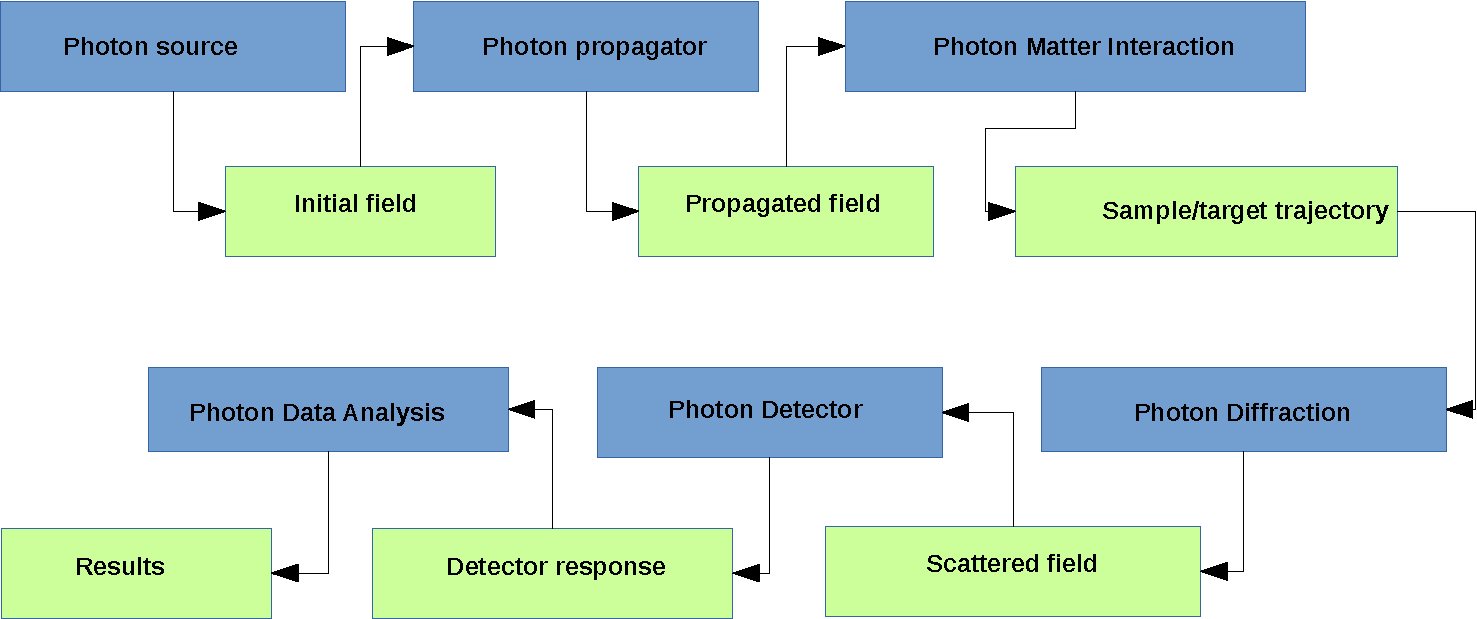
\includegraphics[width=1.0\textwidth,angle=0,clip]{simex_baseline_workflow-crop}
  \end{center}
\caption{Baseline workflow in \texttt{simex\_platform}. Blue boxes represent
\textit{Calculators}, green boxes are data interfaces.}
  \label{fig:simex_baseline_workflow}
\end{figure}

In its current state, \texttt{simex\_platform} supports simulation of
photon experiments, that follow a linear base pattern: The radiation is produced
from a photon source, propagated through a beamline, it interacts with a sample
(target), and photons leaving the sample after scattering or emission are
detected in a photon detector. This linear progression, depicted in
Fig.~\ref{fig:simex_baseline_workflow}, will be referred to as
the simulation  baseline in the following. A typical example is a x-ray diffraction
experiment: X-ray photons delivered by a synchrotron or an FEL, scatter from a
sample (e.g. a crystal), and diffracted photons are captured in
an area detector behind the sample. Other baseline applications are e.g. small
and wide angle scattering, inelastic x-ray scattering, or x-ray absorption
spectroscopy. Simulation of experiments in \texttt{simex\_platform} that are not directly
representable in this ordered linear pattern are possible but not supported in the same way and
to the same extent as baseline applications. For example,
experiments that involve more than one photon source, or applications where
products from photon-matter interaction (e.g. accelerated electrons or ions) are
required for further interactions, such as laser-plasma based short pulse length x-ray and UV sources,
proton radiography and cancer therapy using laser accelerated protons.

A baseline application encapsulates five parts:
The photon source, the photon transport from the source to the
experiment, the interaction of photons and matter, propagation of scattered and
transmitted radiation from the target/sample to the detector, and photon
detection. In \texttt{simex\_platform}
each of these blocks is represented by a suitable \textit{Calculator}. A
\textit{Calculator} can be seen as an operator acting on the data representing
radiation. It reads data from an input, performs a calculation with the data,
potentially modifies the data based on the calculation results, and  writes the
modified or propagated radiation to its output. Calculators are organized in a
lightweight abstraction scheme, represented in Fig.~\ref{fig:simex_calculators_tree}.
\begin{figure}[ht]
  \begin{center}
    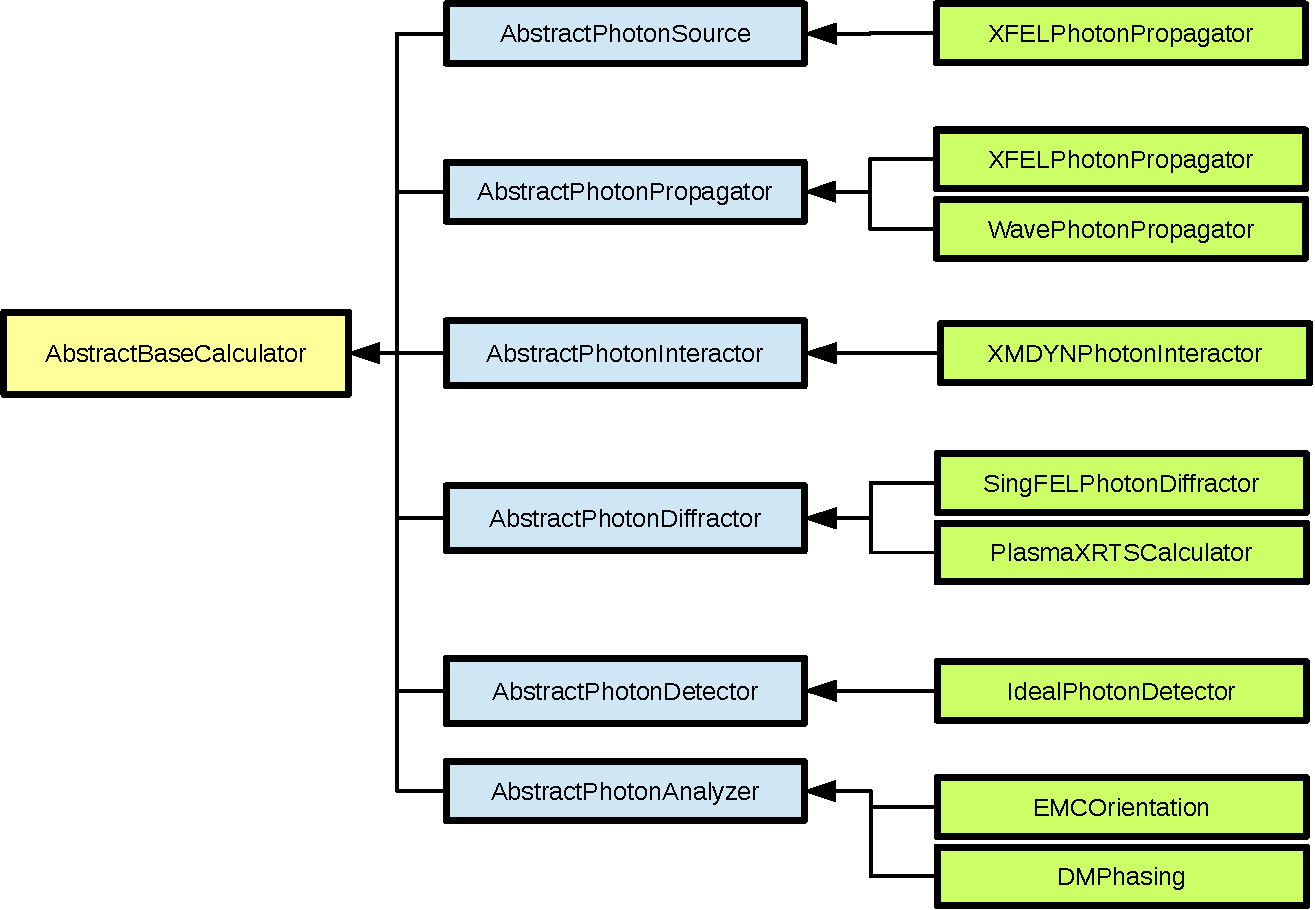
\includegraphics[width=1.0\textwidth,angle=0,clip]{calculators_inheritance-crop}
  \end{center}
  \caption{Inheritance tree for \textit{Calculators} in \texttt{simex\_platform}.}
  \label{fig:simex_calculators_tree}
\end{figure}

Commonalities between calculators are implemented on higher levels of
abstraction (blue or yellow boxes) whereas
specialities of each individual \textit{Calculator} are encapsulated in the
derived classes (green boxes). By providing as much functionality as possible on
the abstract level, the task of adding a new calculator to the set of existing
calculators is facilitated to a large degree, making \texttt{simex\_platform}
user friendly and opening collaborative opportunities, also beyond EUCALL.


\subsection{Interfaces}
Start-to-end simulations in \texttt{simex\_platform} require that any two
subsequent \textit{Calculators} employed in the simulation pipeline can
communicate data amongst each other. The data source has to write the data in a
format that the ensuing data sink can handle and interpret correctly. In
\texttt{simex\_platform}, we chose the Hierarchical Data Format (hdf5) \cite{HDFGroup1997}
as the underlying format for all simulation data files.  Data consistency in the
workflow is realized by each \textit{Calculator} defining the names of hdf
datasets and attributes that it requires to perform its calculation task and the
names of all datasets and attributes that it provides to the subsequent
calculator. In this way, after instantiating the \textit{Calculators} for a
simulation, the user or a workflow manager can check if the data can be
channeled through the \textit{Calculators} and give a feedback if there is a
mismatch between provided and expected data for two subsequent
\textit{Calculators}. This approach is inherited from the preceding simulation
framework \texttt{simS2E} \cite{Yoon2016, simS2Edoc}. Recently, we have started
to adopt a more general approach of defining inter-calculator interfaces based
on the open standard for particle-mesh data \texttt{openPMD}
(\url{www.openpmd.org}).


\subsection{Backengines}
The \textit{Calculators} in \texttt{simex\_platform} are user interfaces to
software executables or scripts that perform the actual mathematical operations on the
\textit{Calculator's} input data. In the following, we refer to these
executables and scripts as the \textit{Backengines}. One \textit{Calculator}
always wraps exactly one \textit{Backengine}, but one \textit{Backengine} can be
wrapped by more than one \textit{Calculator}.


\section{Baseline science applications and required simulation codes}
An intermediate goal in SIMEX is to enable simulation of three distinct baseline
experiments. The following tables list the simulation codes
(\textit{backengines}) that
will be employed for the simulation, as well as relevant references and links to
further details. The linked sections give a brief description of the numerical and physical
methods and specify the data interfaces.
\begin{enumerate}
  \item Single-particle imaging at the European XFEL (SPB-SFX
    instrument)\label{baseline_application_spi}\\
    {\scriptsize%
    \begin{tabular}{l|l|l|l}
      \hline
      \hline
      \textbf{Module} & \textbf{Backengine}
      & \textbf{References} & \textbf{Details} \\
      \hline
      %
      Photon source &  FAST, XPD database &
      \cite{Saldin1999,xpd_xfel} & \ref{sec:interface_source_fast} \\
      %
      Propagation &  WPG/SRW &
      \cite{Samoylova2016, wpg_github} & \ref{sec:interface_prop_wpg} \\
      %
      Photon-Matter Interaction & XMDYNandXATOM
      & \cite{Jurek2016, Son2011, Ziaja2015} & \ref{sec:interface_pmi_xmdyn} \\
      %
      Photon diffraction &  singFEL & \cite{Yoon2016} &
      \ref{sec:interface_diffr_singfel} \\
      %
      Photon detection &  X-CSIT & \cite{Joy2015} &
      \ref{sec:interface_det_xcsit} \\
      %
      %Photon data analysis &  RECON & \cite{Loh2009} &
      %\ref{sec:interface_ana_recon} \\
      \hline
      \hline
    \end{tabular}
  }
  \item Small-angle x-ray scattering from high power laser excited overdense
    plasmas (XFEL, HED instrument)\label{baseline_application_hpl}\\
    {\scriptsize%
    \begin{tabular}{l|l|l|l}
      \hline
      \hline
      \textbf{Module} & \textbf{Backengine}
      & \textbf{References} & \textbf{Details} \\
      \hline
      %
      Photon source &  FAST, XPD database &
      \cite{Saldin1999,xpd_xfel} & \ref{sec:interface_source_fast} \\
      %
      Propagation &  WPG/SRW &
      \cite{Samoylova2016, wpg_github} & \ref{sec:interface_prop_wpg} \\
      %
      Photon-Matter Interaction & PIConGPU
      & \cite{Bussmann2013} & \ref{sec:interface_pmi_picongpu} \\
      %
      Photon scattering &  paraTaxis & \cite{Kluge2016b} &
      \ref{sec:interface_scat_parataxis} \\
      %
      Photon detection &  X-CSIT & \cite{Joy2015} &
      \ref{sec:interface_det_xcsit} \\
      %
      \hline
      \hline
    \end{tabular}
  }

  \item Warm dense matter production through high energy laser shock compression
    and x-ray radiography diagnostics (ESRF, beamline ID24)\label{baseline_application_wdm}\\
    {\scriptsize%
    \begin{tabular}{l|l|l|l}
      \hline
      \hline
      \textbf{Module} & \textbf{Backengine}
      & \textbf{References} & \textbf{Details} \\
      \hline
      %
      Propagation &  Oasys/ShadowUI &
      \cite{Rio2014} & \ref{sec:interface_prop_shadow}\\
      %
      Photon-Matter Interaction & Esther, Multi2D
      & \cite{Colombier2005, Ramis2009} & \ref{sec:interface_pmi_esther} \\
      %
      Radiography & Oasys/ShadowOui & \cite{Rio2014} &
      \ref{sec:interface_prop_shadow} \\
      \hline
      \hline
    \end{tabular}
  }

\end{enumerate}
%
\section{Listing of SIMEX \textit{Backengines}, and interfaces}
This section gives more detailed information about the simulation codes used in
SIMEX, their data interfaces as well as graphical representations of simulation data to demonstrate their
functionality.
\subsection{Photon source }
\subsubsection{FAST\label{sec:interface_source_fast}}
\begin{description}
  \item[Method:] 3D time resolved explicit solver
  \item[Domain:] SASE FEL simulation
  \item[Data structure:]\ \\
    {\scriptsize%
   \begin{tabular}{l|l}
      \hline
      \hline
      /data/arrEhor     & horizontal electric field component \\
      /data/arrEver     & vertical electric field component \\
      /params/Mesh/nSlices    & number of time slices \\
      /params/Mesh/nx     & number of grid points in horizontal dimension (x) \\
      /params/Mesh/ny     & number of grid points in vertical dimension (y) \\
      /params/Mesh/sliceMax     & time corresponding to last slice \\
      /params/Mesh/sliceMin     & time corresponding to first slice \\
      /params/Mesh/xMax     & x coordinate of last grid point in horizontal dimension \\
      /params/Mesh/xMin     & x coordinate of first grid point in horizontal dimension \\
      /params/Mesh/yMax     & y coordinate of last grid point in vertical dimension \\
      /params/Mesh/yMin     & y coordinate of first grid point in vertical dimension \\
      /params/Mesh/zCoord     & z coordinate of the wavefront \\
      /params/Rx    &  instantaneous horizontal wavefront radius\\
      /params/Ry    &  instantaneous vertical wavefront radius\\
      /params/dRx     & error in Rx \\
      /params/dRy     & error on Ry \\
      /params/nval    &  data type of field values, 2 for complex \\
      /params/photonEnergy    & central photon energy (mean of spectrum) \\
      /params/wDomain     & time or frequency domain\\
      /params/wEFieldUnit     & Electric field unit \\
      /params/wFloatType    &  field numerical type \\
      /params/wSpace      &  direct (r-space) or reciprocal (q-space)\\
      /params/xCentre     & x coordinate of wavefront center \\
      /params/yCentre     & y coordinate of wavefront center \\
      /history/parent/info/data\_description     & data documentation \\
      /history/parent/info/package\_version    & code version \\
      /history/parent/misc/FAST2XY.DAT    &  \\
      /history/parent/misc/angular\_distribution     & angular distribution of source pulse \\
      /history/parent/misc/spot\_size    & fhwm spot size \\
      /history/parent/misc/gain\_curve     & gain curve \\
      /history/parent/misc/nzc    & Undulator length (point on gain curve0 \\
      /history/parent/misc/temporal\_struct    & Temporal pulse structure (on-axis projection) \\
      \hline
      \hline
    \end{tabular}
      }
    \item[Example data:]\ \\[2ex]
        \begin{center}
          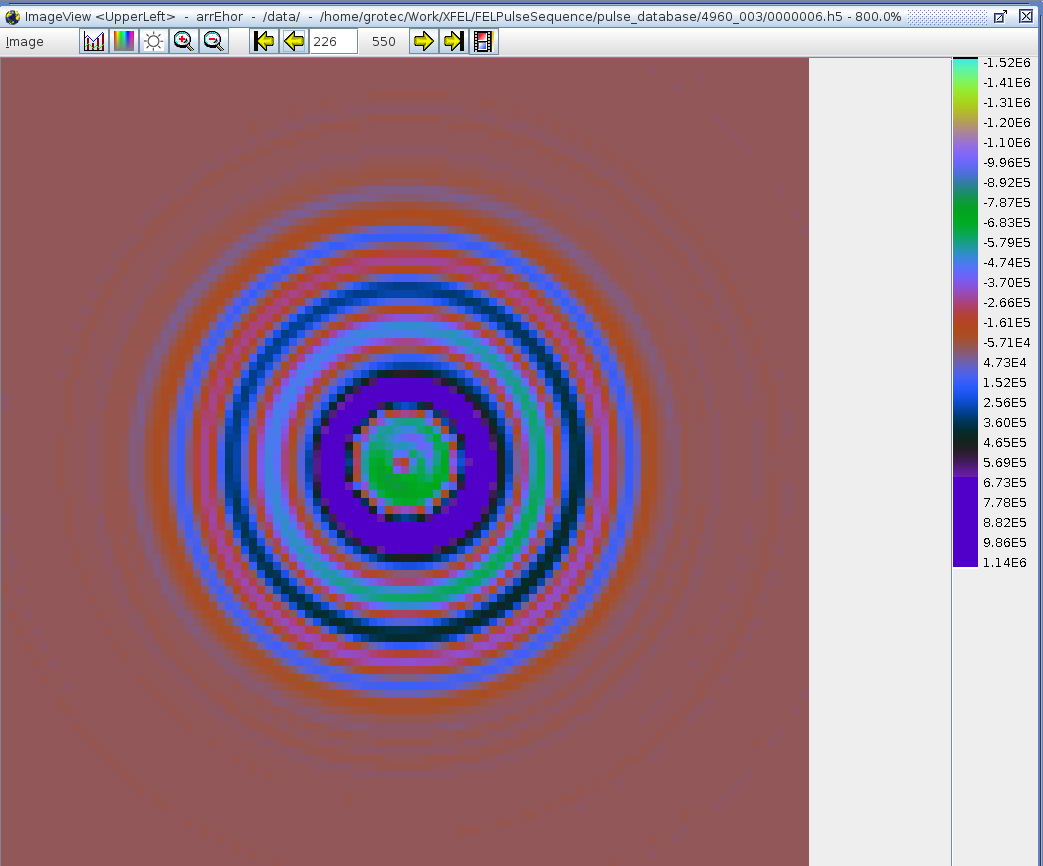
\includegraphics[width=0.5\textwidth,angle=0,clip]{figures/felsource_demo}
        \end{center}
        \scriptsize{FEL source calculation using the code FAST: Horizontal
        component of electric field distribution near pulse center in a plane perpendicular to
      propagation direction at undulator exit in SASE 1 beamline at the European
      XFEL \cite{xpd_xfel}.}
    \end{description}

%\subsubsection{ESRF source code \label{sec:interface_esrf_source_code}}
%\begin{description}
  %\item[Method:] ??
  %\item[Data structure:] ??
%\end{description}
%
\subsection{Photon Propagation (Task 4.1.1)}
Propagates the radiation as described by the photon source calculator from the
source to the point of interaction with the sample or target under
investigation. Describes focussing, filtering, pulse shaping, and other optical
effects realized through lenses, mirrors, apertures, grids etc.
\subsubsection{WPG/SRW\label{sec:interface_prop_wpg}}
\begin{description}
  \item[Method:] Fourier optical wave propagation
  \item[Data structure:]\ \\
{\scriptsize%
\begin{tabular}{l|l}
  \hline
  \hline
  /data/arrEhor     & horizontal electric field component \\
  /data/arrEver     & vertical electric field component \\
  /params/Mesh/nSlices    & number of time slices \\
  /params/Mesh/nx     & number of grid points in horizontal dimension (x) \\
  /params/Mesh/ny     & number of grid points in vertical dimension (y) \\
  /params/Mesh/qxMax        & x coordinate of last q-grid point in horizontal
  dimension \\
  /params/Mesh/qxMin        & x coordinate of first q-grid point in horizontal
  dimension \\
  /params/Mesh/qyMax        & y coordinate of last q-grid point in vertical dimension \\
  /params/Mesh/qyMin        & y coordinate of first q-grid point in vertical
  dimension \\
  /params/Mesh/sliceMax     & time corresponding to last slice \\
  /params/Mesh/sliceMin     & time corresponding to first slice \\
  /params/Mesh/xMax     & x coordinate of last grid point in horizontal dimension \\
  /params/Mesh/xMin     & x coordinate of first grid point in horizontal dimension \\
  /params/Mesh/yMax     & y coordinate of last grid point in vertical dimension \\
  /params/Mesh/yMin     & y coordinate of first grid point in vertical dimension \\
  /params/Mesh/zCoord     & z coordinate of the wavefront \\
  /params/Rx    &  instantaneous horizontal wavefront radius\\
  /params/Ry    &  instantaneous vertical wavefront radius\\
  /params/dRx     & error in Rx \\
  /rtreparams/dRy     & error on Ry \\
  /params/nval    &  data type of field values, 2 for complex \\
  /params/photonEnergy    & central photon energy (mean of spectrum) \\
  /params/wDomain     & time or frequency domain\\
  /params/wEFieldUnit     & Electric field unit \\
  /params/wFloatType    &  field numerical type \\
  /params/wSpace    &  direct (r-space) or reciprocal (q-space)\\
  /params/xCentre     & x coordinate of wavefront center \\
  /params/yCentre                 & y coordinate of wavefront center \\
  /info/package\_version          & WPG version \\
  /info/contact        & Support contact details \\
  /info/data\_description         & Data documentation \\
  /info/method\_description       & Method documentation \\
  /misc/xFWHM        & Full width at half maximum of the intensity distribution in horizontal dimension\\
  /misc/yFWHM        & Full width at half maximum of the intensity distribution in
  vertical dimension\\
  /version        & Interface version \\
  \hline
  \hline
\end{tabular}
}
\item[Example data:]\ \\
      \begin{center}
        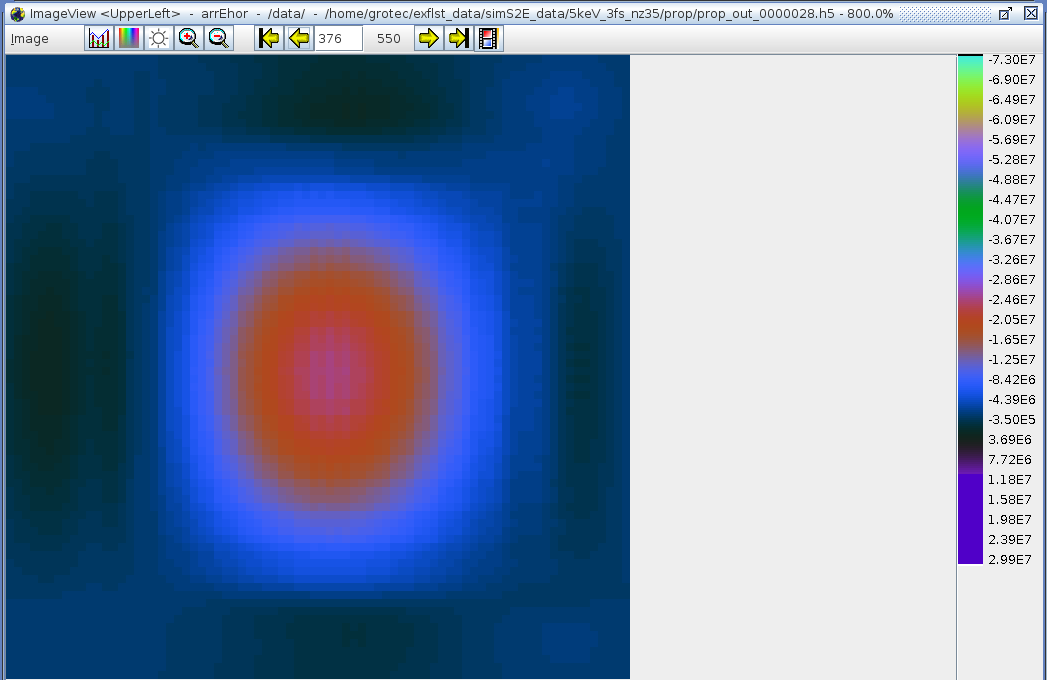
\includegraphics[width=0.5\textwidth,angle=0,clip]{figures/wpg_demo}
      \end{center}
      \scriptsize{Propagation of source wavefront as calculated by WPG: Horizontal
      component of electric field distribution near pulse center in plane perpendicular to
    propagation direction at sample positon in the SPB-SFX instrument at
    European XFEL.}
\end{description}

%
\subsubsection{Oasys\label{sec:interface_prop_shadow}}
\begin{description}
  \item[Method:] X-ray raytracing
  \item[Domain:] Synchrotron radiation propagation
  \item[Data structure:] See Ref.~\cite{Rio2014}
  \item[Example data:] See Ref.~\cite{Rio2014}
\end{description}
%
\subsection{Photon Interactor (Task 4.1.2)}
Interaction of the photons with the target or sample. Takes into account
elementary processes like absorption, emission, scattering of radiation and
secondary processes like collisional ionization and recombination. The end
product is the electronic state of the sample/target as a function of time
during the interaction with the external light source.
\subsubsection{XMDYNandXATOM\label{sec:interface_pmi_xmdyn}}
\begin{description}
  \item[Method:] Molecular Dynamics and Hartree-Fock electronic structure
  \item[Domain:] Atoms and Molecules in intense x-ray fields
  \item[Data structure:]\ \\
{\scriptsize%
\begin{tabular}{l|l}
  \hline
  \hline
  /data/snp*/ff        & 2D array of form factors. Rows: Atomic number, Columns: q  \\
  /data/snp*/halfQ        & 1D array of half-period resolutions corresponding to
  column index in form factor arrays \\
  /data/snp*/Nph        & number of photons in the calculation \\
  /data/snp*/r        & 2D array of atomic position vectors. Rows: Atom index,
  columns: x,y,z coordinates \\
  /data/snp*/T        & 1D array of unique ID per atomic number \\
  /data/snp*/Z        &  1D array of atom types per atomic position vector
  $r$\\
  /data/snp*/xyz        & 1D array of indices of ff for each atom in Z \\
  /data/snp*/Sq\_halfQ        & half period resolution q space spanned by
  Sq\_bound, Sq\_free \\
  /data/snp*/Sq\_bound        & 1D array for Compton scattering from bound electrons \\
  /data/snp*/Sq\_free        & 1D array for Compton scattering from free
  electrons \\
  /history/parent/detail        & Input parameters used to run the code \\
  /info/package\_version        & backengine code version \\
  /info/contact        & Support contact for backengine code \\
  /info/data\_description        & Data documentation \\
  /info/method\_description        & Method documentation \\
  /version                   & hdf5 format version \\
  \hline
  \hline
\end{tabular}
}
\item[Example data:]\ \\
      \begin{center}
        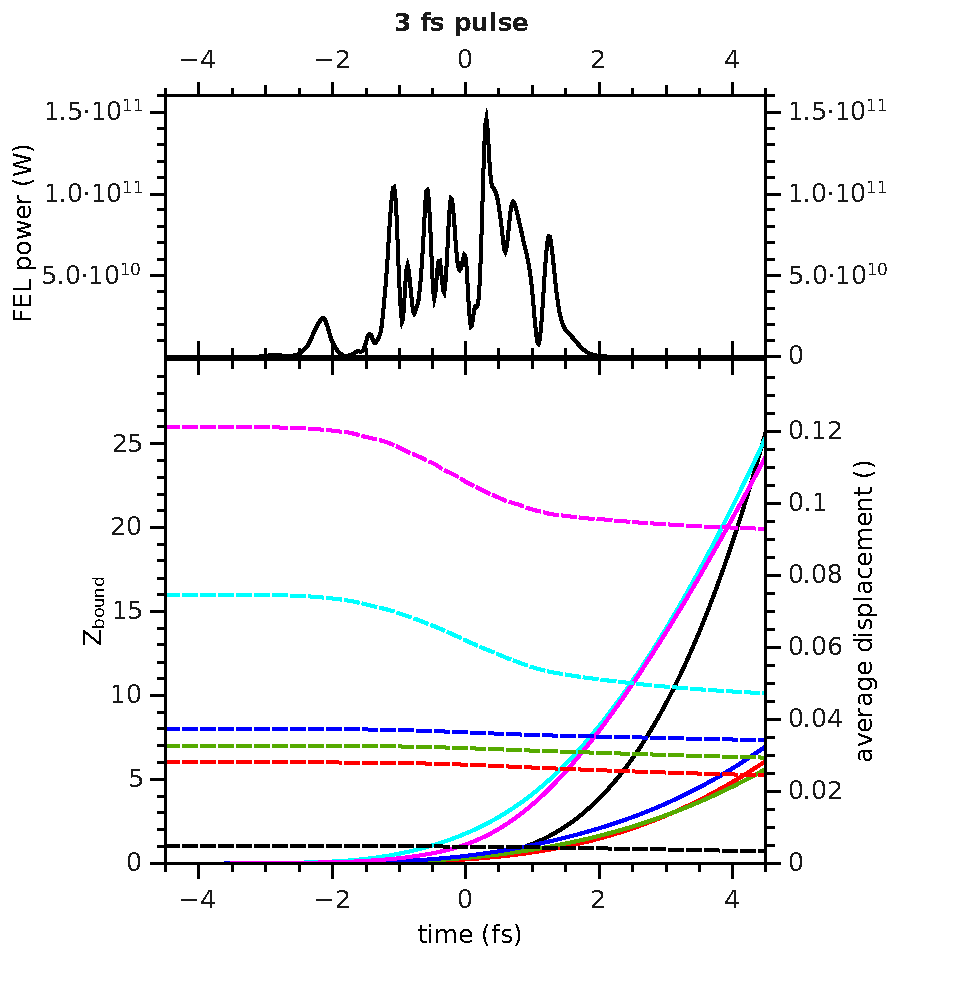
\includegraphics[width=0.5\textwidth,angle=0,clip]{pmi_3fs.pdf}
      \end{center}
      \scriptsize{Photon-matter calculation using XMDYNandXMATOM:
        3 fs XFEL pulses (5 keV photon energy) (power vs time, top panel), average displacement, and average ionization
        (bottom) for the irradiated 2NIP molecule \cite{Schlessman1998, Fortmann-Grote2016b}.}
\end{description}
%
\subsubsection{PIConGPU\label{sec:interface_pmi_picongpu}}
\begin{description}
  \item[Method:] 3D3V Particle-In-Cell (PIC)
  \item[Data structure:] openPMD incl. domain extension for PIC.
  \item[Example data:]\ \\
      \begin{center}
        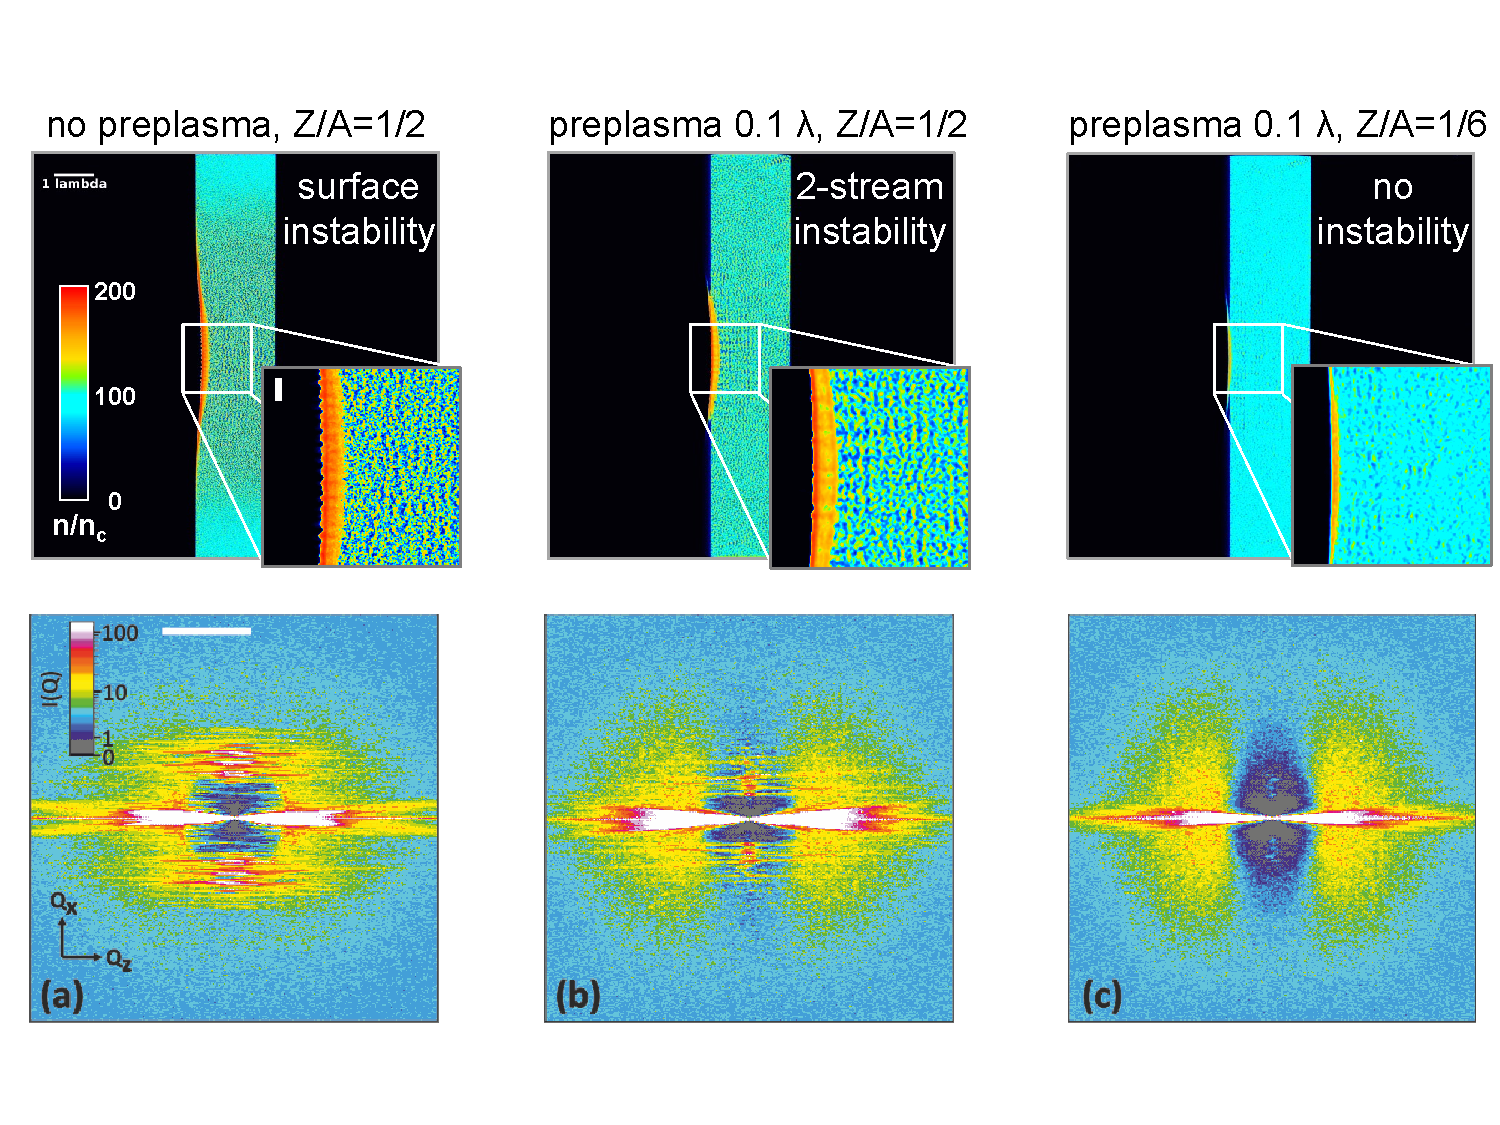
\includegraphics[width=0.5\textwidth,angle=0,clip]{bussmann_saxs_instabilities.pdf}
      \end{center}
      \scriptsize{PIConGPU calculations of electron density (top) and
        corresponding Small Angle X-ray Scattering signals (bottom) from high power laser -- matter
    interaction.}
\end{description}
%
\subsubsection{Esther\label{sec:interface_pmi_esther}}
\begin{description}
  \item[Method:] 1-D radiation hydrodynamics
  \item[Domain:] Dynamic compression
  \item[Data structure:] openPMD
  \item[Example data:] \ \\
    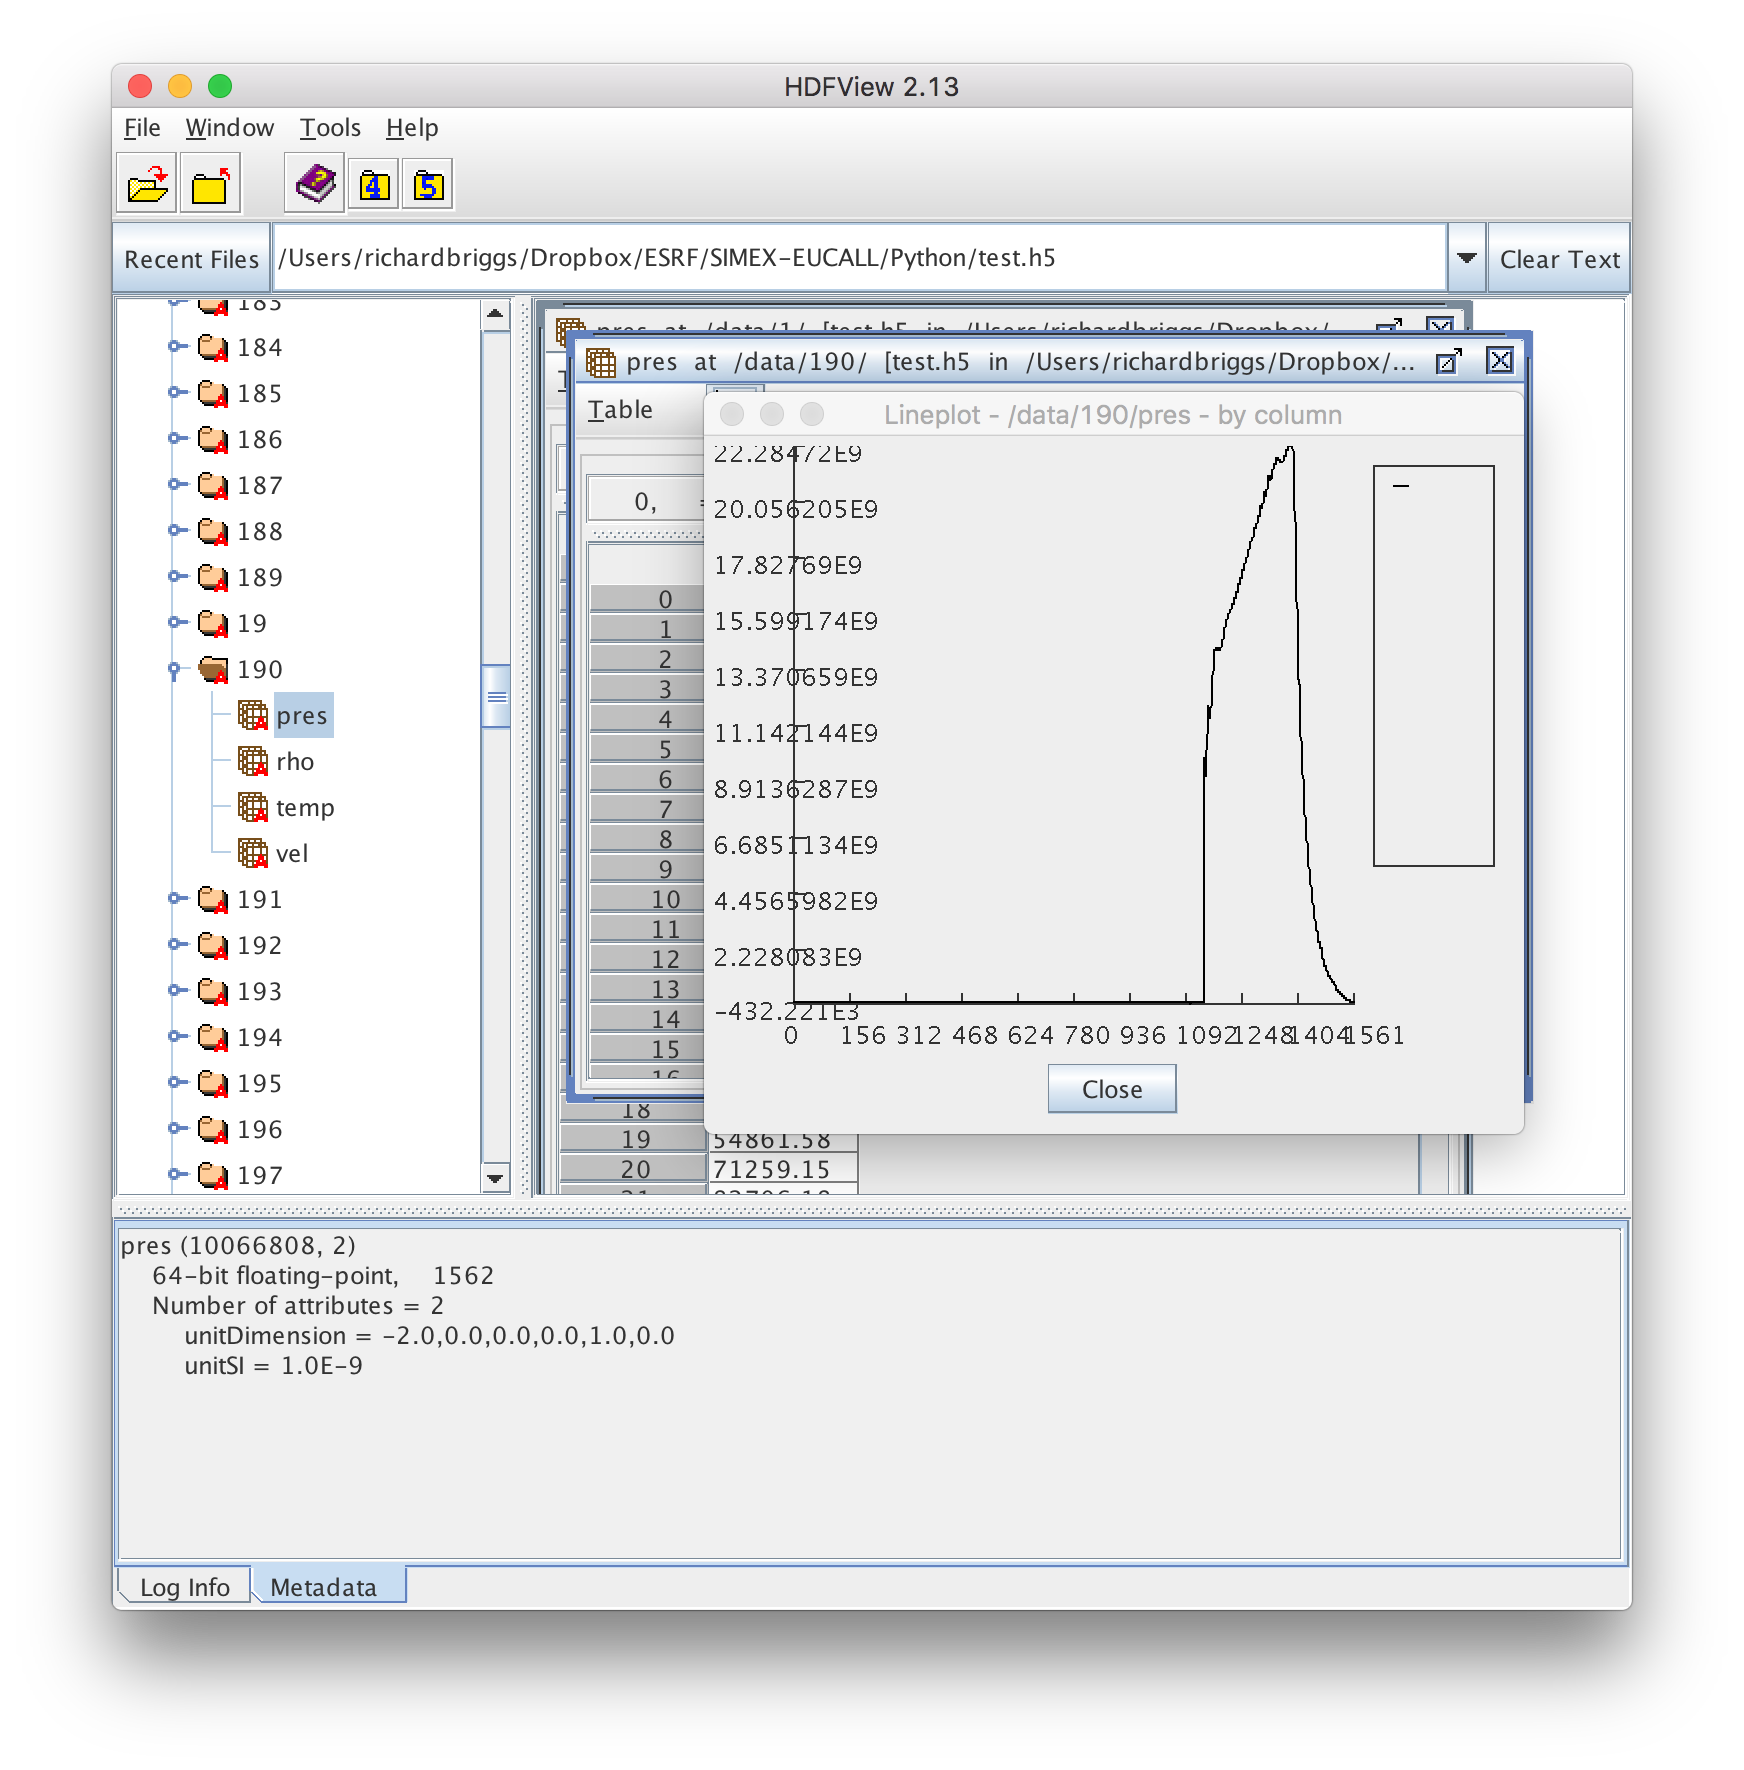
\includegraphics[width=0.5\textwidth,angle=0,clip]{esther_demo}\\
    \scriptsize{Shock front simulation using Esther: Pressure vs. distance after
    high energy -- solid matter (iron) interaction.}
\end{description}

%\subsection{Photon Scattering and Diffraction (Task 4.1.3)}
%\subsubsection{\textbf{Code for XAFS simulation}\label{sec:interface_xafs_code}}
%\begin{description}
  %\item[Method:] ??
  %\item[Domain:]
  %\item[Data structure:] ??
%\end{description}

\subsubsection{paraTaxis\label{sec:interface_scat_parataxis}}
\begin{description}
  \item[Method:] MonteCarlo tracking of individual photons
  \item[Domain:] Ex-situ and in-situ photon scattering from strongly excited
    plasmas
  \item[Data structure:] openPMD particles
  \item[Demonstraction data:] See \ref{sec:interface_pmi_picongpu}
\end{description}

\subsubsection{singFEL\label{sec:interface_diffr_singfel} }
\begin{description}
  \item[Method:] 2nd order Born approximation scattering using electronic form factors.
  \item[Data structure:]\ \\
{\scriptsize%
  \begin{tabular}{l|l}
    \hline
    \hline
/data/data        & 2D array. Integrated intensity per pixel \\
/data/diffr        & 2D array. Integrated intensity converted to photon count
(Poissonized) \\
/data/angle        & Euler angles applied to atomic positions \\
/history/parent/detail        &  Details of parent data\\
/history/parent/parent        & Parent data, hierarchical \\
/info/package\_version        & Backengine code version \\
/info/contact        & Support contact \\
/info/data\_description        & Data documentation \\
/info/method\_description        & Method documentation \\
/params/geom/detectorDist        & Detector distance \\
/params/geom/pixelWidth        & Pixel width (x) \\
/params/geom/pixelHeight        & Pixel height (y) \\
/params/geom/mask        & Masked pixels \\
/params/beam/photonEnergy        & Central photon energy  \\
/params/beam/photons        & Number of photons in beam \\
/params/beam/focusArea        & Beam focus area \\
/params/info        & Input parameter for backengine code \\
\hline
\hline
\end{tabular}
}
    \item[Example data:]\ \\
      \begin{center}
        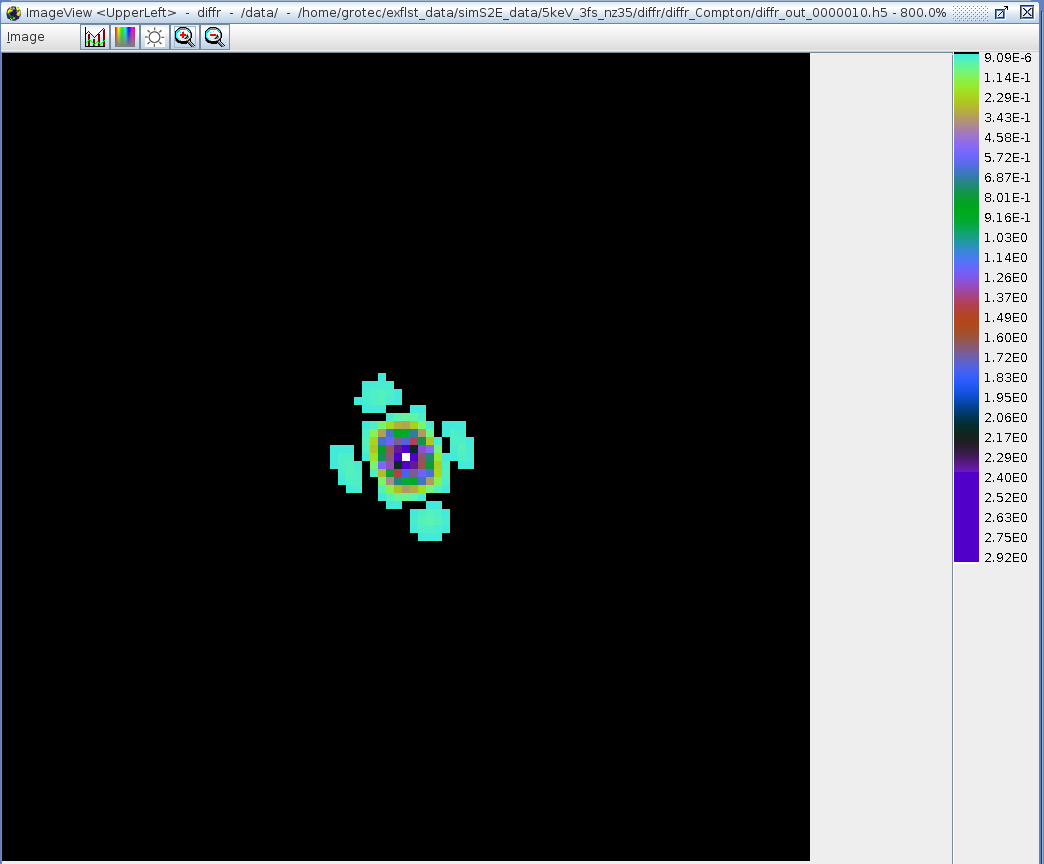
\includegraphics[width=0.5\textwidth,angle=0,clip]{diffr_demo}
      \end{center}
      \scriptsize{Simulated diffraction intensity distribution using singFEL. }
\end{description}
%
\subsubsection{XRTS code\label{sec:interface_scat_xrts}}
\begin{description}
  \item[Method:] 2nd Born approximation for differential inelastic scattering cross section for scattering from warm and hot dense plasmas in various
    approximations \cite{Gregori2006a, Fortmann2009d, Fortmann2010a}
  \item[Domain:] X-ray Thomson Scattering in Dense Plasmas
  \item[Data structure:]\ \\
{\scriptsize%
  \begin{tabular}[ ]{l|l}
    \hline
    \hline
    /data/dynamic/Skw\_bound & Bound electron Compton scattering structure factor \\
    /data/dynamic/Skw\_free &  Free electron scattering structure factor\\
    /data/dynamic/Skw\_total & Total scattering structure factor \\
    /data/dynamic/energy\_shifts & Range of energy shifts spanned by dynamic
    structure factors \\
    /data/static/Sk\_core     & Core electron static structure factor \\
    /data/static/Sk\_free      & Free electron static structure factor \\
    /data/static/Sk\_ion           & Ion static structure factor \\
    /data/static/Sk\_total         & Total static structure factor \\
    /data/static/Wk               & Ion feature $|f+q|^2 S_{ii}(k)$ \\
    /data/static/debye\_waller     & Debye-Waller factor \\
    /data/static/fk               & Atomic form factor $f(k)$ \\
    /data/static/ipl              & Ionization potential lowering \\
    /data/static/lfc              & Local field factor \\
    /data/static/qk               & Screening cloud $q(k)$ \\
    \hline
    \hline
  \end{tabular}
}
\item[Example data:]\ \\
      \begin{center}
        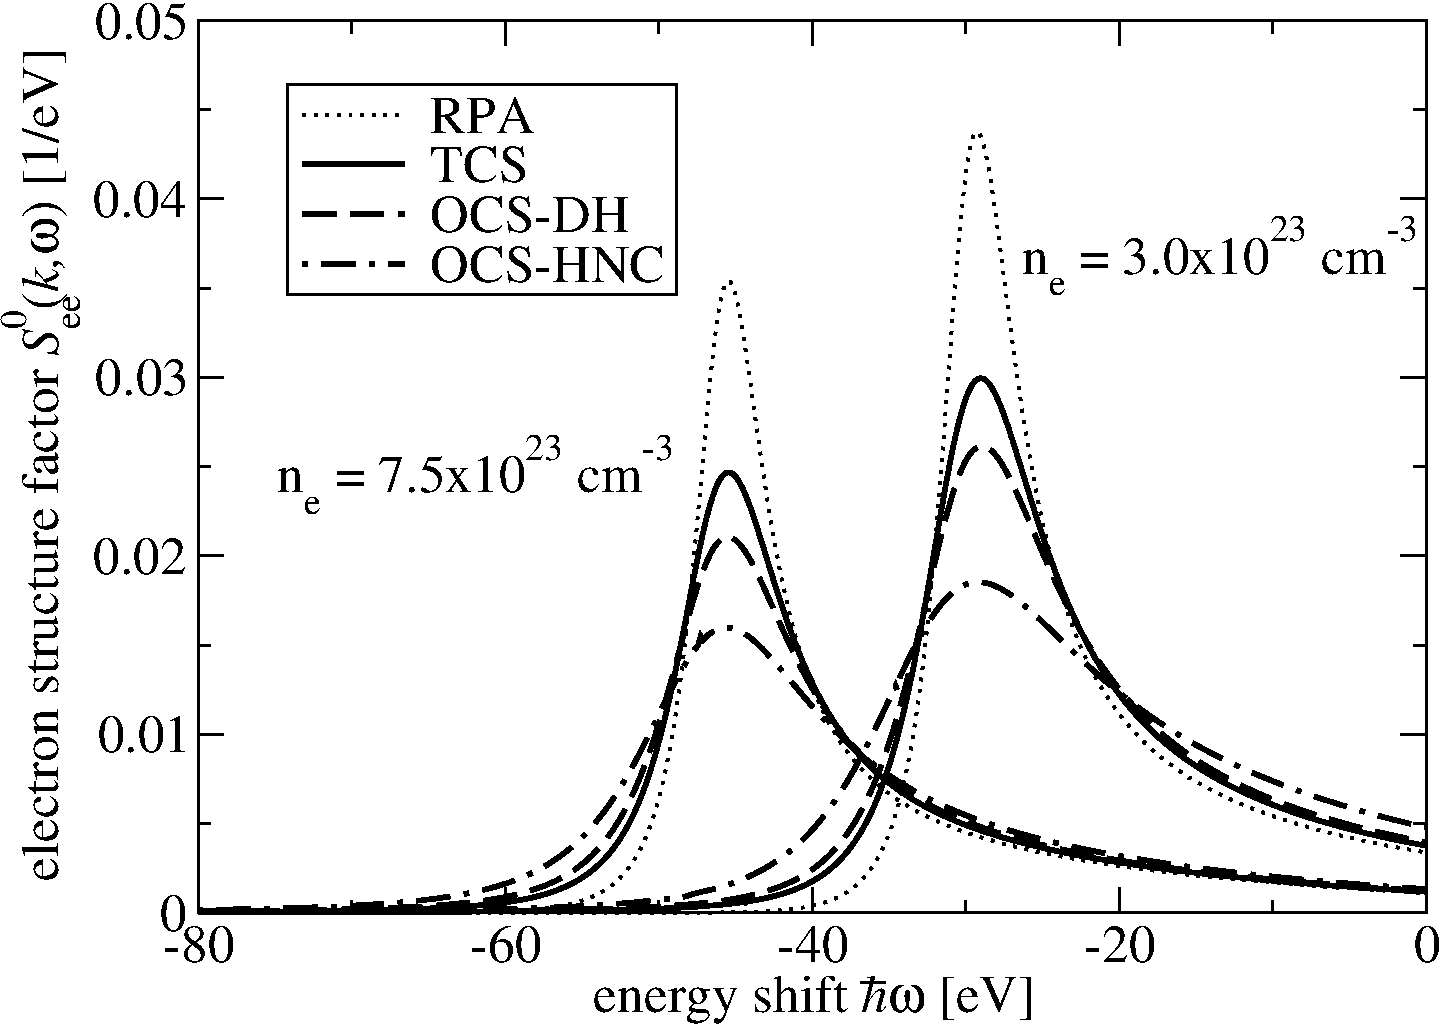
\includegraphics[width=0.5\textwidth,angle=0,clip]{Skw_TCS-DH-RPA.pdf}
      \end{center}
      \scriptsize{Simulated X-ray Thomson Scattering spectra using various ion-ion
      structure factor models for two electron densities. Scattered intensity as
    function of energy shift, simulated with XRTS code.}
\end{description}
%
\subsection{Photon Detector (Task 4.1.4)}
\subsubsection{X-CSIT\label{sec:interface_det_xcsit}}
\begin{description}
  \item[Method:] Combined particle, charge, and electronics simulation
  \item[Domain:] Pixel area detectors
  \item[Data structure:]\ \\
{\scriptsize%
  \begin{tabular}{l|l}
    \hline
    \hline
/data/diffr        & 2D array. Photon count per pixel
(Poissonized) \\
/history/parent/detail        &  Details of parent data\\
/history/parent/parent        & Parent data, hierarchical \\
/info/package\_version        & Backengine code version \\
/info/contact        & Support contact \\
/info/data\_description        & Data documentation \\
/info/method\_description        & Method documentation \\
/params/geom/detectorDist        & Detector distance \\
/params/geom/pixelWidth        & Pixel width (x) \\
/params/geom/pixelHeight        & Pixel height (y) \\
/params/geom/mask        & Masked pixels \\
/params/beam/photonEnergy        & Central photon energy  \\
/params/beam/photons        & Number of photons in beam \\
/params/beam/focusArea        & Beam focus area \\
/params/info        & Input parameter for backengine code \\
\hline
\hline
\end{tabular}
}
\item[Example data:] See Ref.~\cite{Joy2015}.
\end{description}
%
\newpage
%
\printbibliography
%
%%%%%%%%%%%%%%%%%%%%%%%
\end{document}


